\subsection{Система кинематического управления}\label{part_kinematic_control}

Кинематическое управление реализуется в два этапа: первый включает в себя получение траектории движения сочленений манипулятора $ \bm{q}(t) $ или схвата $ \bm{s}(t) $ на интервале времени $ t \in [t_s,\,\,t_f] $; второй этап подразумевает синтез системы управления, способной отработать спланированную траекторию.

Планированию траекторий посвящён следующий раздел. Здесь реализуем систему управления для следования по заданной траектории.

\begin{figure}[h!]
	\centering{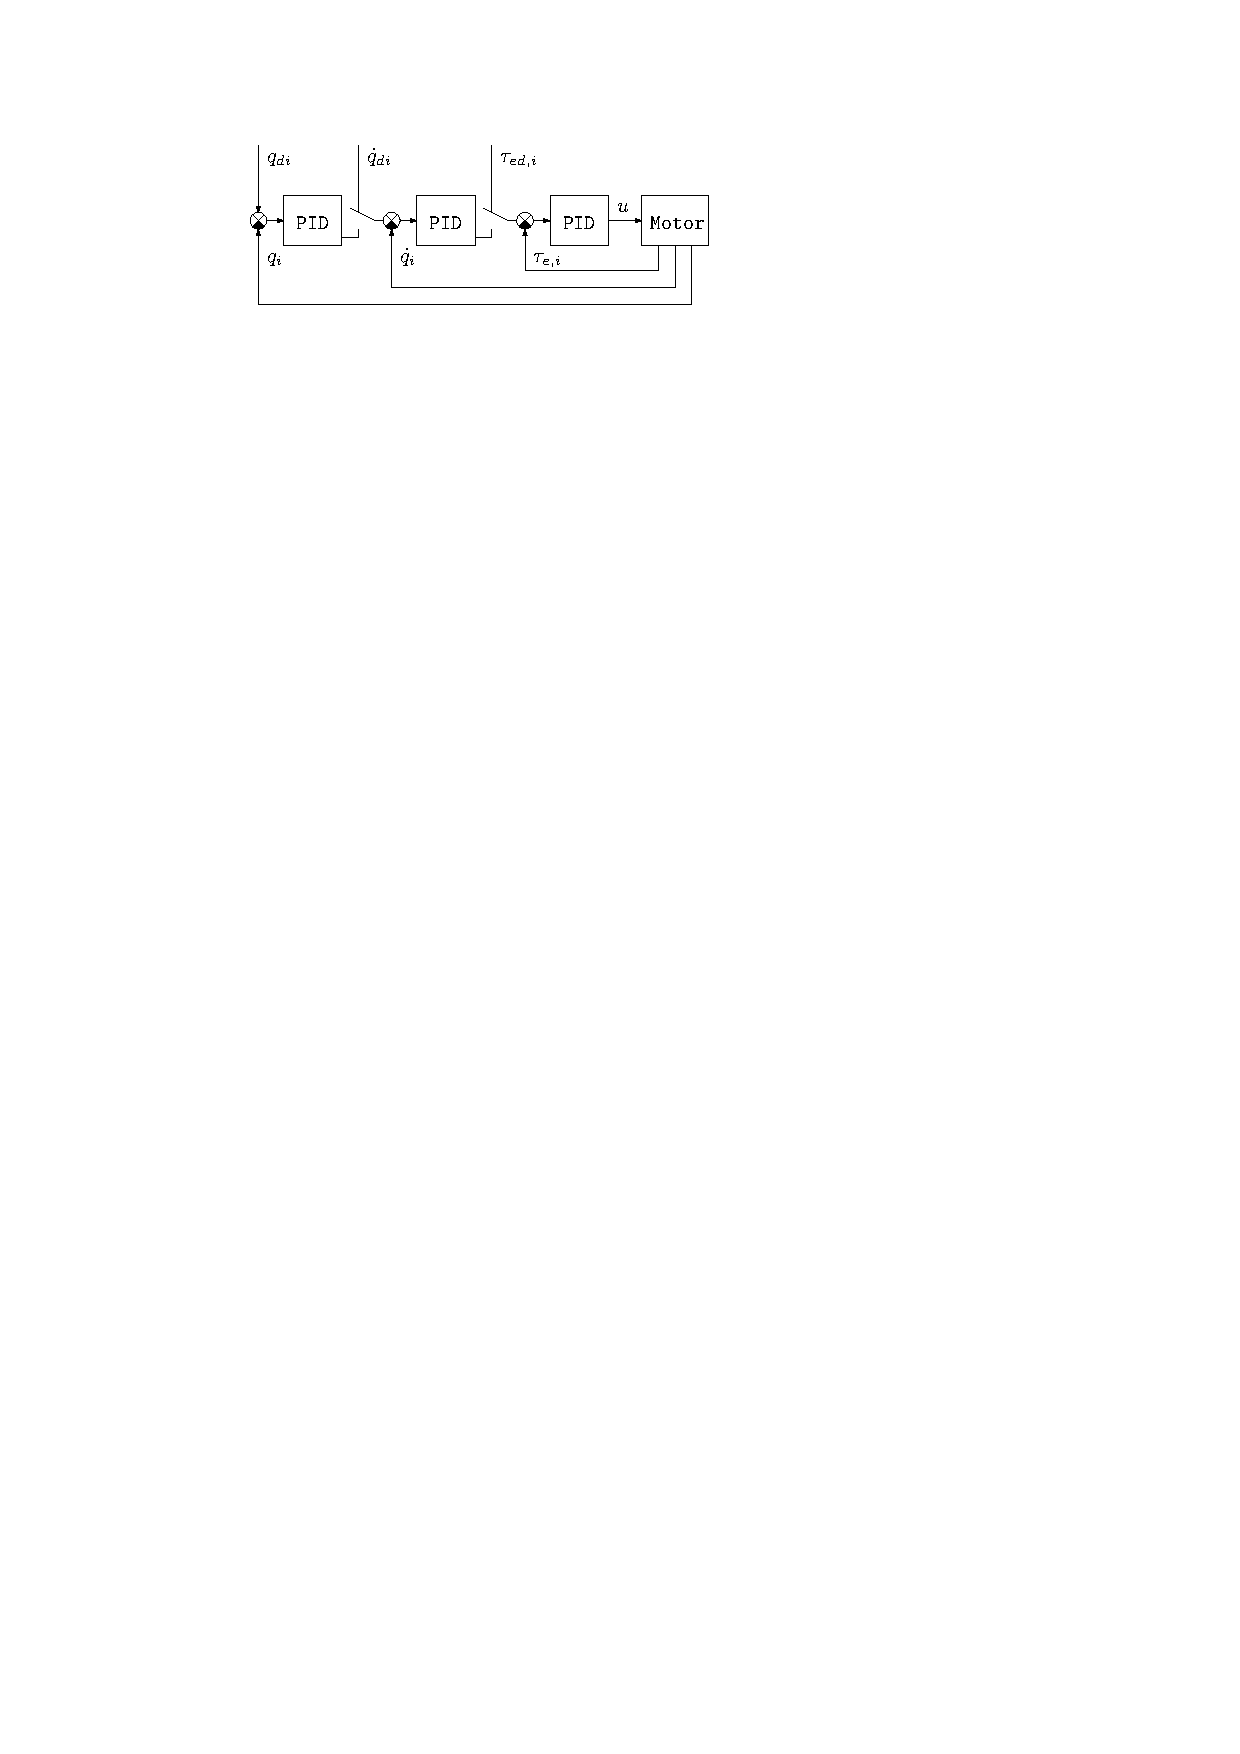
\includegraphics[width=0.7\textwidth]{structure_of_actuator_cs.pdf}}
	\vspace{0.5cm}
	\caption{Структурная схема системы управления приводами, встроенная в контроллеры манипулятора}
	\label{img:structure_of_actuator_cs}
\end{figure}

Каждый из приводов манипулятора робота KUKA Youbot имеет собственную систему управления, структура которой иллюстрируется схемой, представленной на рисунке~\ref{img:structure_of_actuator_cs}. Из нее видно, что каждый из приводов робота может управляться заданием значения для угла $ q_{di} $, или скорости $ \dot{q}_{di} $, или момента силы $ \tau_{ed,i} $, который должен быть на нем обеспечен. Это значение подается на вход соответствующего ПИД-регулятора, коэффициенты которого доступны настройке, и далее (уже в виде сигнала напряжения u) на контролируемый двигатель.

Далее в тексте будет рассмотрена система управления, в которой в качестве управляющего сигнала рассматриваются векторы $ \bm{q} $ и $ \dot{\bm{q}} $. Из величин, описывающих состояние робота в данный момент времени, в используемом ПО доступны векторы $\bm{q}(t)$, $\dot{\bm{q}}(t)$ и $\bm\tau_e (t)$.

Цель управления в минимизации ошибки между заданной траекторией и положением схвата в каждый момент времени. Введём обозначения: траекторию обозначим, как:
\begin{equation}
	\bm{s}_d = 
	\begin{bmatrix}
		\bm p_d \\
		\bm\varphi_d
	\end{bmatrix}
	= f(\bm{q}_d),
	\quad
	\dot{\bm{s}}_d = 
	\begin{bmatrix}
		v_d \\
		\omega_d
	\end{bmatrix}
	 = f(\dot{\bm{q}}_d),
\end{equation}
а текущее положение схвата:
\begin{equation}
	\bm{s} = 
	\begin{bmatrix}
		\bm p \\
		\bm\varphi
	\end{bmatrix}
	= f(\bm{q}),
	\quad
	\dot{\bm{s}} = 
	\begin{bmatrix}
		v \\
		\omega
	\end{bmatrix}
	= f(\dot{\bm{q}}),
\end{equation}

%%%\textcolor{red}{Расчёт текущего положения схвата осуществляется методом Ньютона, который касательные и все такое, описанного в~\ref{part_newton}. ДОБАВИТЬ ЧАСТЬ В РЕШЕНИЕ ЗАДАЧ КИНЕМАТИКИ!!1}

%%%%%%%%%%%%%%%
%\textbf{Управление по вектору скорости.}

Для следования по траектории, заданной функциями $ \bm{s}_d(t) $ и  $ \dot{\bm{s}}_d(t) $ реализуем управление по вектору скорости, которое формулируется как минимизация ошибки скорости следования по траектории. Воспользуемся соотношением для обратной задачи о скорости:
\begin{equation}
	\dot{\bm{q}} = J^+(q) \dot{\bm{s}},
\end{equation}
где $ \bm{q} $~--- вектор обобщенных координат, $ \bm{s} $~--- вектор, определяющий положение схвата, $ J^+ $~--- псевдообратная матрица (так как размерность матрицы Якоби для рассматриваемого манипулятора $[6\times 5]$).

Введем ошибку по положению схвата:
\begin{equation}\label{error}
	\bm{e}(t) = \bm{s}_d(t) - \bm{s}(t).
\end{equation}
Затем, дифференцируя~\eqref{error} по времени, получим:
\begin{equation}
	\dot{\bm{e}}(t) = \dot{\bm{s}}_d(t) - \dot{\bm{s}}(t) =
	\dot{\bm{s}}_d(t) - J^+(q) \dot{\bm{q}}.
\end{equation}
Необходимо выбрать вектор $ \dot{\bm{q}}(t) $ таким, чтобы выполнялось условие
\begin{equation}
	\lim_{t\to\infty} \dot{\bm{e}}(t) = 0.
\end{equation}
Тогда, если
\begin{equation}
	\dot{\bm{q}}(t) = J^+(q) \cdot (\dot{\bm{s}}_d(t) - \dot{\bm{e}}(t)),
\end{equation}
то, выбрав 
\begin{equation}
	\dot{\bm{e}}(t) = - K {\bm{e}}(t),
\end{equation}
можно обеспечить асимптотическую устойчивость системы управления.

Схема системы управления изображена на рисунке~\ref{img:velocity_control_system}.
\begin{figure}[h!]
	\centering{\includegraphics[width=1\textwidth]{ipe/velocity_control_system.pdf}}
	\caption{Система управления по вектору скорости}
	\label{img:velocity_control_system}
\end{figure}

В следующем разделе рассмотрим способы задания траектории, которую в последствии будем подавать на вход синтезированной системы управления.

